% Drawing 74/05-9 -- folder 74, batch 05, archive page 83 (PDF page 84).
% Transcription: Diagramme esquissé : $\mathrm{Car}_{s}=\mathrm{hex}_{d}\longrightarrow\mathrm{Car}_{s,\mathrm{ép}}$, avec $\wr$ vers $\mathrm{tria\,ép}$ et $\mathrm{Hex\,ép}$ ; puis $\mathrm{Car}_{\wedge}\simeq\mathrm{hex}_{d}\longleftarrow\mathrm{Car}_{p'}\simeq\mathrm{hex}_{s*}$, $\wr\ \simeq\mathrm{hex}^{*}_{d}$, « \uncertain{tri pav.\ pet} » ; $\mathrm{Car}\simeq$ \uncertain{pav.\ pet.} ; $\mathrm{Car}_{d*}$, $\mathrm{Car}_{s*}$ ; chaque terme accompagné de petits schémas (triangles, segments pointillés, cadres).
% Kind: sketched arrow diagram with small schemas. Method 2 (schematic redraw from the facsimile). Status: partial.
% Notes: Car_s = hex_d -> Car_{s,ép}, with wr down to tria ép and Hex ép; Car_wedge = hex_d <- Car_p' = hex_s*, wr = hex*_d, « tri pav. pet » (uncertain); Car = pav. pet. (uncertain); Car_d*; and, at the end of the long arrow from Car_d*, a label read Car_s* (the transcription's Car_s*, its index overinked). Labels at \small (the figure drawn at 1.4 mm per unit), placed where they stand. Each term has a small schema beside it (framed triangles, a framed square, hatched frames, points); these are drawn as outlines with their marked points, and their inner strokes are approximate. The square of arrows at the bottom right is 05-10, and the three shapes at the top right are 05-8. Still differs: the inner strokes and hatching of the small schemas (the hatched frame by Car_d* and the one at the right are drawn as outlines with their bold strokes only). Redrawn 2026-11-09 (issue 128): to check again. Overlay check 2026-11-13 (issue 147, Claude claude-opus-5-5): the redraw, rasterised by the skill's previewer (not compiled: no TeX in the session), laid over the 300 dpi colour crop of the scan (261 ppi). The terms, the arrows and the small schemas lie on their ink to within 1 to 3 units. Still differs, as said above: the inner strokes and the hatching of the small schemas are drawn as outlines with their bold strokes only. It is an arrow diagram, which the editor prefers set as LaTeX (tikz-cd or array) in the transcription; as a redraw it stays partial.
% Coordinates: 1 unit = 1.4 mm = 1/100 of the crop width (bbox in page fractions: [0.08, 0.5, 0.75, 0.85]).
% Redrawn by Claude (claude-opus-5-5), issue #73, 2026-11-09; not checked by a human; not compiled (no TeX in the session).
% Checked by Claude (claude-opus-5-5) 2026-11-13 (issue #147): overlaid on the 300 dpi colour facsimile; not compiled (no TeX in the session). Status: partial.
% Rights: reproduces part of the work -- behind RENDER_TRANSCRIPTS, never published by itself.
\documentclass[tikz,border=3pt]{standalone}
\usepackage{amsmath,amssymb}
\usetikzlibrary{patterns,arrows.meta}
\tikzset{pencil/.style={black!45}, struck/.style={black!35}, mark/.style={circle,draw,inner sep=1.3pt}, pt/.style={circle,fill,inner sep=0.9pt}, opt/.style={circle,draw,fill=white,inner sep=1.1pt}}
\begin{document}
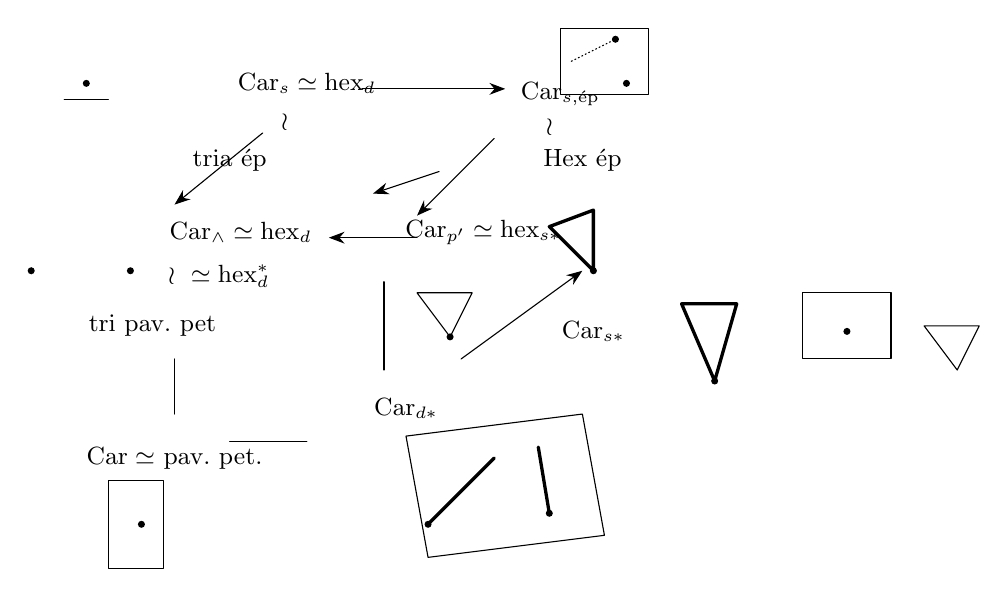
\begin{tikzpicture}[x=1.4mm,y=1.4mm,line cap=round,line join=round,font=\scriptsize]
\node[inner sep=1pt] at (37,-15) {\small $\mathrm{Car}_s\simeq\mathrm{hex}_d$};
\draw[-{Stealth[length=2mm]}] (42,-15.5) -- (55,-15.5);
\node[inner sep=1pt] at (60,-16) {\small $\mathrm{Car}_{s,\mathrm{\acute ep}}$};
\node[inner sep=1pt] at (35,-18.5) {\small $\wr$};
\node[inner sep=1pt] at (59,-19) {\small $\wr$};
\node[inner sep=1pt] at (30,-22) {\small tria ép};
\node[inner sep=1pt] at (62,-22) {\small Hex ép};
\node[inner sep=1pt] at (31,-28.5) {\small $\mathrm{Car}_\wedge\simeq\mathrm{hex}_d$};
\draw[-{Stealth[length=2mm]}] (47,-29) -- (39,-29);
\node[inner sep=1pt] at (53,-28.5) {\small $\mathrm{Car}_{p'}\simeq\mathrm{hex}_{s*}$};
\node[inner sep=1pt] at (29,-32.5) {\small $\wr\ \simeq\mathrm{hex}^*_d$};
\node[inner sep=1pt] at (23,-37) {\small tri pav.\ pet};
\node[inner sep=1pt] at (25,-49) {\small $\mathrm{Car}\simeq$ pav.\ pet.};
\node[inner sep=1pt] at (46,-44.5) {\small $\mathrm{Car}_{d*}$};
\draw[-{Stealth[length=2mm]}] (33,-19.5) -- (25,-26);
\draw[-{Stealth[length=2mm]}] (54,-20) -- (47,-27);
\draw[-{Stealth[length=2mm]}] (49,-23) -- (43,-25);
\draw[-{Stealth[length=2mm]}] (51,-40) -- (62,-32);
\draw (25,-40) -- (25,-45);
\draw (44,-33) -- (44,-41);
\draw (30,-47.5) -- (37,-47.5);
\node[pt] at (17,-15) {};
\draw (15,-16.5) -- (19,-16.5);
\node[pt] at (12,-32) {};
\node[pt] at (21,-32) {};
\draw (60,-10) -- (68,-10) -- (68,-16) -- (60,-16) -- cycle;
\draw[densely dotted] (61,-13) -- (65,-11);
\node[pt] at (65,-11) {};
\node[pt] at (66,-15) {};
\draw[very thick] (59,-28) -- (63,-26.5) -- (63,-32) -- cycle;
\node[pt] at (63,-32) {};
\draw (47,-34) -- (52,-34) -- (50,-38) -- cycle;
\node[pt] at (50,-38) {};
\draw[very thick] (71,-35) -- (76,-35) -- (74,-42) -- cycle;
\node[pt] at (74,-42) {};
\draw (82,-34) -- (90,-34) -- (90,-40) -- (82,-40) -- cycle;
\node[pt] at (86,-37.5) {};
\draw (93,-37) -- (98,-37) -- (96,-41) -- cycle;
\draw (46,-47) -- (62,-45) -- (64,-56) -- (48,-58) -- cycle;
\draw[very thick] (48,-55) -- (54,-49);
\draw[very thick] (58,-48) -- (59,-54);
\node[pt] at (48,-55) {};
\node[pt] at (59,-54) {};
\draw (19,-51) -- (24,-51) -- (24,-59) -- (19,-59) -- cycle;
\node[pt] at (22,-55) {};
\node[inner sep=1pt] at (63,-37.5) {\small $\mathrm{Car}_{s*}$};
\end{tikzpicture}
\end{document}
